% $Header$

\documentclass{beamer}

% This file is a solution template for:

% - Giving a talk on some subject.
% - The talk is between 15min and 45min long.
% - Style is ornate.



% Copyright 2004 by Till Tantau <tantau@users.sourceforge.net>.
%
% In principle, this file can be redistributed and/or modified under
% the terms of the GNU Public License, version 2.
%
% However, this file is supposed to be a template to be modified
% for your own needs. For this reason, if you use this file as a
% template and not specifically distribute it as part of a another
% package/program, I grant the extra permission to freely copy and
% modify this file as you see fit and even to delete this copyright
% notice. 


\mode<presentation>
{
  %\usetheme{Warsaw}
  %\usetheme{Berlin}
  %\usetheme{metropolis}
  \usetheme{PaloAlto}
  %\usetheme{CambridgeUS}
  %\usetheme{Berkeley}
  
  % font themes
  \usefonttheme{serif}
  %\usefonttheme{structurebold}

  % color themes
  %\usecolortheme{albatross}
  %\usecolortheme{beetle}
  %\usecolortheme{crane}
  %\usecolortheme{dove}
  %\usecolortheme{fly}
  %\usecolortheme{monarca}
  %\usecolortheme{seagull}
  %\usecolortheme{beaver}
  % color themes
  % or ...

  %\setbeamercovered{transparent}
  \setbeamercovered{transparent=5}
  % or whatever (possibly just delete it)
}


\usepackage[english]{babel}
% Place figures exactly where you mean to
%https://tex.stackexchange.com/a/8633/64425
\usepackage{float}
% Place figures exactly where you mean to
% or whatever

\usepackage[utf8]{inputenc}
% or whatever

\usepackage[T1]{fontenc}
% Or whatever. Note that the encoding and the font should match. If T1
% does not look nice, try deleting the line with the fontenc.

% math
\usepackage{amsmath}
\usepackage{amssymb}
\usepackage{amsthm}
% math

% tikz
\usepackage{tikz}
\usetikzlibrary{arrows.meta}
\usetikzlibrary{calc}
% tikz
\usepackage{caption}
\usepackage{hyperref}
\hypersetup{
    colorlinks,
    linkcolor={magenta!50!black},
    citecolor={blue!50!black},
    urlcolor={blue!80!black}
}
% large commented sections
\usepackage{comment}
% large commented sections

% some beautiful fonts
\usepackage{yfonts}
% some beautiful fonts

% canceling in equations
\usepackage{cancel}
% canceling in equations

\title[Nonstandard Analysis] % (optional, use only with long paper titles)
{Nonstandard Analysis, The 1972-SciAm Article}

\subtitle
{Ideas That Common People Brand Nonstandard} % (optional)

\author[MD,RH,KM] % (optional, use only with lots of authors)
{Martin Davis\inst{1} \and Reuben Hersh\inst{2}}
% - Use the \inst{?} command only if the authors have different
%   affiliation.

\institute[Unknown] % (optional, but mostly needed)
{
  \inst{1}%
  Original Author
  \and
  \inst{2}%
  Original Author
  }
% - Use the \inst command only if there are several affiliations.
% - Keep it simple, no one is interested in your street address.

\date[August 2025] % (optional)
{Aug 2025 / Free Learner's School Conversations}

\subject{Fun Conversations at Home School}
% This is only inserted into the PDF information catalog. Can be left
% out. 



% If you have a file called "university-logo-filename.xxx", where xxx
% is a graphic format that can be processed by latex or pdflatex,
% resp., then you can add a logo as follows:

% \pgfdeclareimage[height=0.5cm]{university-logo}{university-logo-filename}
% \logo{\pgfuseimage{university-logo}}



% Delete this, if you do not want the table of contents to pop up at
% the beginning of each subsection:
\AtBeginSubsection[]
{
  \begin{frame}<beamer>{Outline}
    \tableofcontents[currentsection,currentsubsection]
  \end{frame}
}


% If you wish to uncover everything in a step-wise fashion, uncomment
% the following command: 

%\beamerdefaultoverlayspecification{<+->}


\begin{document}

\begin{frame}
  \titlepage
\end{frame}

\begin{frame}{Outline}
  \tableofcontents
  % You might wish to add the option [pausesections]
\end{frame}


% Since this a solution template for a generic talk, very little can
% be said about how it should be structured. However, the talk length
% of between 15min and 45min and the theme suggest that you stick to
% the following rules:  

% - Exactly two or three sections (other than the summary).
% - At *most* three subsections per section.
% - Talk about 30s to 2min per frame. So there should be between about
%   15 and 30 frames, all told.

% [Kedar] I am keeping this structure, but abusing it to serve my purpose.
% [Kedar] I expect this `presentation' to have many hundred slides, if I end up doing it right.
% [Kedar] There are three sections per presentation, no subsections, but each section may have many, many slides. Let's see. I am just getting started with LaTeX and Beamer.
% [Kedar] I may roughly make a chapter in his book a section in this presentation.
\section{Introduction}
\begin{frame}
\frametitle{Nonstandard Analysis}
\framesubtitle{Common Words, Uncommon Meanings, Yet Again!}
\label{slide:nonstd-anal}
\begin{itemize}
\pause
\item This Is A Review of A Davis-Hersh\footnote{Both Were Mathematicians with a Gift of Writing Extraordinary Expository Articles.} Article in Scientific American, June 1972.
\begin{itemize}
\pause
\item You Perhaps Haven't Even Heard \alert{``Nonstandard Analysis''} in The Context of Calculus-1.
\pause
\item \alert{Analysis} Refers to \alert{Foundations of Calculus}.
\item \alert{Nonstandard} Only Because The Word \alert{`Standard' Was Taken} to Mean Formalization of Calculus Using Some Other (Beautiful) Way!
\end{itemize}
\pause
\item These Slides Are A Gentle Introduction to Nonstandard Analysis, Are for Personal Benefit, Only Indirectly for Actual Presentation.
\pause
\item There's No Need to Get Intimidated by \alert{Big Words}.
\pause
\item Let's Be Fearless in Guided Imagination, and Make \alert{Inquiry} A Habit.
\end{itemize}
\end{frame}

\begin{frame}
\frametitle{A Bit of History}
\framesubtitle{Everything Has A History!}
\label{slide:history-of-nonstandard-analysis}
\begin{itemize}
\item Influential Ancient Greeks, Euclid, Aristotle, \& Archimedes, \alert{Avoided The \textit{Unthinkable} Infinity (Infinitely Large) \& The \textit{Strange} Infinitesimals (Infinitely Small)}. 
\pause
\item Ideas of Calculus Over Time Culminated into \alert{Leibniz's and Newton's Formulation of Calculus} in The 1680s.
\pause
\item Both Used The \alert{\textit{Banned} Infinitesimals}:
\begin{itemize}
\pause
\item Small, \alert{Infinitely Small} Non-Archimedean Numbers!
\pause
\item Smaller Than Any Finite Number, Yet Bigger Than 0!
\end{itemize}
\pause
\item Several Philosophers/Mathematicians Criticized\footnote{Prominent Among Them Was Bishop George Berkeley, The Famous Clergyman for Whom the University of Berkeley, California is Named!} Leibniz and Newton for These \textit{Infinitesimal Numbers} \alert{That Exist in A Sort of Neverland}!
\pause
\item Infinitesimals Defied \alert{Logic Prevalent at The Time}!
\pause
\item And So, Karl Weierstrass et. al. \alert{Banished Infinitesimals from Calculus by The 1890s}!
\end{itemize}
\end{frame}

\begin{frame}
\frametitle{A Bit More of History}
\framesubtitle{Everything Has A History!}
\label{slide:more-history-of-nonstandard-analysis}
\begin{itemize}
\pause
\item Weierstrass Formalized Calculus Using The Allegedly Non-intuitive Idea of \alert{Limits}.
\pause
\item However, In 1966, The Logician Abraham Robinson Reintroduced Infinitesimals And Provided The \alert{Necessary Rigor} to Them!
\pause
\item Several Mathematicians Criticized Robinson's Work!
\pause
\item But in 2020s, It Is Considered Original Body of Work That Is \alert{Equivalent To Standard Analysis}; Strangely, Logic Prevalent Now Necessitates Infinitesimals!
\pause
\item In The End, Your Approach to Calculus Reduces to \alert{Your Philosophy of Mathematics}: Choice Is Yours!
\pause
\item The War between \alert{The Continuous And The Discrete} Is Reignited.
\end{itemize}
\end{frame}

\begin{frame}
\frametitle{Does That Make You Uncomfortable?}
\framesubtitle{Be My Guest!}
\label{slide:uncomfortable}
\begin{itemize}
\pause
\item On The First Encounter, \alert{Nonstandard Analysis Feels, Well, \textit{Nonstandard}}!
\pause
\item It Makes Us \alert{Ponder The Nature of Mathematics}.
\pause
\item Although It Stretches Our Imagination, Its Logic And Equivalence with Standard Analysis Is \alert{Fun}!
\begin{itemize}
\pause
\item After All, When \textit{Applied to Practical Problems}, Both Approaches \alert{Produce Exactly The Same Results}!
\end{itemize}
\end{itemize}
\end{frame}

\begin{frame}
\frametitle{}
\framesubtitle{}
\label{slide:infinitesimal-in-geometry}
\begin{block}{Geometry}
Let's Introduce Infinitesimals in Geometry.
\end{block}
\end{frame}

% ------ copypasta next 5 ------
\begin{frame}
\frametitle{The Area And Circumference of The Unit Circle}
\framesubtitle{Argument 1: A \textit{Logically Unacceptable} Argument Based on Infinitesimals}
\label{slide:rejected-by-euclid}
\begin{columns}[c]
\begin{column}{.7\textwidth}
\begin{proof}[Area of Unit Circle = $\frac{1}{2}$ Its Circumference ({\tiny Would Euclid Accept It?})]
Any circle can be thought of as composed of \alert{infinitely many straight-line segments, all equal to each other and infinitely short}.  It is then the sum of \alert{infinitesimal triangles}, all of which have altitude 1. Area of a triangle = half the base times the altitude. Therefore, the sum of the areas of the triangles is half the sum of the bases. But the sum of the areas of the triangles is the area of the circle, and the sum of the bases of the triangles is its circumference. \alert{Therefore, the area of the unit circle = half its circumference}.
\end{proof}
\end{column}
\begin{column}{0.3\textwidth}
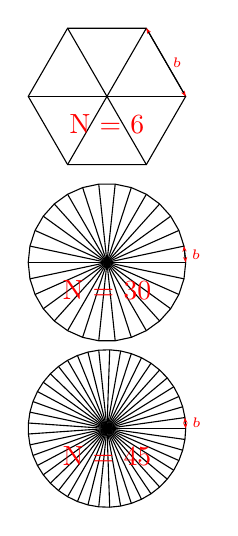
\begin{tikzpicture}
\def\r{1}
\def\N{10}
\foreach \N / \Y in {6/0,30/60,45/120} {
  \def\ang{360/\N}
  \def\ys{-\Y}
  \draw [yshift=\ys] let \n1 = {360/\N}, \n2 = {2*\n1}, \n{N-1} = {360 - \n1} in
  (0:\r) foreach \a in {\n1,\n2,...,\n{N-1}} {-- (\a:\r)} -- cycle;
  
  \foreach \x in {0,1,2,...,\N}
    \draw [yshift=\ys] (0:0) -- (\x*\ang:\r);
  
  \node [yshift=\ys-10,color=red] {N = \N};
  \draw [{Stealth[length=2pt,red]}-{Stealth[length=2pt,red]}][yshift=\ys] (0:\r) -- node[xshift=4,red] {{\tiny $b$}} (\ang:\r);
}
\end{tikzpicture}
\end{column}
\end{columns}
\end{frame}
% ------ copypasta prev 5 ------

\begin{frame}
\frametitle{Seriously?}
\framesubtitle{Is That (\alert{Argument 1} [\ref{slide:rejected-by-euclid}]) A Valid Mathematical Proof?}
\label{slide:objections-to-nic}
\begin{itemize}
\pause
\item That \textit{Argument} [\ref{slide:rejected-by-euclid}] Was Published by \alert {Nicholas of Cusa in The $15^{th}$ Century}!
\pause
\item We Wonder If It Is Even Logical! Clearly, \alert{Objections Galore}!
\begin{itemize}
\pause
\item The \alert{Very Notion of A Triangle with An Infinitely Small Base Is Illusive}!
\pause
\item The Base of The Triangle, $b$, \alert{However Small}, Must Clearly Be $\geq0$, Right?
\pause
\begin{enumerate}
\item If $b=0$, \alert{No Number of Triangles Can Make A Circle with Positive Circumference}!
\item If $b>0$, \alert{Infinitely Many Triangles Make An Infinitely Large Circumference}!
\end{enumerate}
\pause
\item In Either Case, How Can We Ever Get \alert{A Finite Circle from Infinite Infinitely Small Pieces}?
\begin{enumerate}
\pause \item Every Real Number Must Be Archimedean!
\pause \item Since \alert{No Infinitesimal Is Archimedean}, They Were Rejected by Euclid, Aristotle, Archimedes.
\end{enumerate}
\end{itemize}
\end{itemize}
\end{frame}

\begin{frame}
\frametitle{Archimedes's Work: Lost And Found}
\framesubtitle{Riddle of The Quadrature of The Parabola}
\label{slide:archimedes-method}
\begin{itemize}
\pause
\item \alert{Archimedes's Work Came in Two Streams of Tradition}: 1) Continuous, 2) After A Gap of 1000 Years.
\pause
\item Of Present Interest Is His \alert{Method of Exhaustion}.
\begin{itemize}
\pause
\item Discovered in Constantinople in 1906!
\pause
\item Relies on \alert{An ``Indirect Argument''} And \alert{Purely Finite Constructions}.
\pause
\item Finds The Volumes of \alert{Surfaces of Revolution} (e.g., A Paraboloid).
\pause
\item Since \alert{Infinitesimals Don't Exist\footnote{Or Do They?}}, It Gives A Logically Acceptable, Rigorous Proof of His Results!
\begin{enumerate}
\pause
\item No References Are Made to \alert{Infinitesimals} in It.
\pause
\item Ironically, You May Find Its Logic Akin to \alert{Weierstrass's} Formulation.
\end{enumerate}
\end{itemize}
\end{itemize}
\end{frame}

\begin{frame}
\frametitle{The Area And Circumference of The Unit Circle}
\framesubtitle{Argument 2: A \textit{Logical, But Pedantic,} Argument Avoiding Infinitesimals\alert{?}}
\label{slide:arg-2-archimedes-1}
\begin{proof}[Area of Unit Circle = $\frac{1}{2}$ Its Circumference ({\tiny Flawless Logic?})]
\let\qed\relax % Temporarily removes the QED symbol
Let \alert{$S$} Be The Proposition\footnote{Therefore, $S$ Must Be Either \texttt{true} Or \texttt{false}.} That \alert{The Area of A Unit Circle ($\mathbb{A}_C$) = Its Half-circumference ($\mathbb{H}_C$)}.

\alert{If} $S$ Is \texttt{false}, \alert{Then} 
\begin{equation}
\label{eq:ac-hc}
\text{Either}\quad\mathbb{A}_C>\mathbb{H}_C\quad\text{Or}\quad\mathbb{H}_C>\mathbb{A}_C
\end{equation}

Let $\mathbb{D}$ Be The \textit{Positive Difference} between $\mathbb{A}_C$ And $\mathbb{H}_C$.

Therefore, If $\mathbb{H}_C>\mathbb{A}_C$, Then

\begin{equation}
\label{eq:d=hc-ac}
\mathbb{D}=\mathbb{H}_C-\mathbb{A}_C
\end{equation}

Otherwise,
\begin{equation}
\label{eq:d=ac-hc}
\mathbb{D}=\mathbb{A}_C-\mathbb{H}_C
\end{equation}

\end{proof}
\end{frame}

\begin{frame}
\frametitle{The Area And Circumference of The Unit Circle}
\framesubtitle{Argument 2: Continued \dots}
\label{slide:arg-2-archimedes-2}
\begin{proof}[Area of Unit Circle = $\frac{1}{2}$ Its Circumference ({\tiny Flawless Logic?})]
\let\qed\relax % Temporarily removes the QED symbol
\dots

Now We Use \alert{Proof by Contradiction} to Show that Both Eq. [\ref{eq:d=hc-ac}] and Eq. [\ref{eq:d=ac-hc}] Lead to Contradiction with Eq. [\ref{eq:ac-hc}]. 

Let's start with Eq. [\ref{eq:d=hc-ac}] first.

We Can \alert{Circumscribe @ The Circle A Regular Polygon with as Many Sides as We Wish}.

Since The Polygon Is Composed of Finite Number of Finite Triangles with Altitude = 1, \alert{Area of The Polygon equals Its Half-perimeter}.
\begin{equation}
\label{eq:ap=hp}
\mathbb{A}_P=\mathbb{H}_P
\end{equation}

As The Number of Sides of The Polygon Circumscribing The Circle Increases, The Difference in Their Areas, $\mathbb{A}_P-\mathbb{A}_C$, Reduces.
%We Can Increase The Number of Sides of The Polygon Such That $\mathbb{A}_P-\mathbb{A}_C<\frac{\mathbb{D}}{2}$
\end{proof}
\end{frame}

\begin{frame}
\frametitle{The Area And Circumference of The Unit Circle}
\framesubtitle{Argument 2: Continued \dots}
\label{slide:arg-2-archimedes-3}
\begin{proof}[Area of Unit Circle = $\frac{1}{2}$ Its Circumference ({\tiny Flawless Logic?})]
\let\qed\relax % Temporarily removes the QED symbol
\dots

We Can Increase The Number of Sides of The Polygon Such That $\mathbb{A}_P-\mathbb{A}_C<\frac{\mathbb{D}}{2}$

Then, from Equations [\ref{eq:d=hc-ac}] and [\ref{eq:ap=hp}],
\begin{equation}
\begin{aligned}
\mathbb{H}_P-(\mathbb{H}_C-\mathbb{D})&<\frac{\mathbb{D}}{2}\\
\therefore\mathbb{H}_P-\mathbb{H}_C+\mathbb{D}&<\frac{\mathbb{D}}{2}\\
\therefore\mathbb{H}_P&<\mathbb{H}_C-\frac{\mathbb{D}}{2}
\end{aligned}
\end{equation}

This Is A Contradiction; The Polygon Circumscribes The Circle, How Can Its Perimeter Be Smaller Than That of The Circle?

\end{proof}
\end{frame}

\begin{frame}
\frametitle{The Area And Circumference of The Unit Circle}
\framesubtitle{Argument 2: Continued \dots}
\label{slide:arg-2-archimedes-4}
\begin{proof}[Area of Unit Circle = $\frac{1}{2}$ Its Circumference ({\tiny Flawless Logic?})]
\let\qed\relax % Temporarily removes the QED symbol
\dots

We Reason Similarly for Eq. [\ref{eq:d=ac-hc}]: Increase The Number of Sides of The Polygon Such That $\mathbb{H}_P-\mathbb{H}_C<\frac{\mathbb{D}}{2}$ (Note: Half-Perimeters).  Then, from Equations [\ref{eq:d=ac-hc}] and [\ref{eq:ap=hp}],
\begin{equation}
\begin{aligned}
\mathbb{A}_P-(\mathbb{A}_C-\mathbb{D})&<\frac{\mathbb{D}}{2}\\
\therefore\mathbb{A}_P-\mathbb{A}_C+\mathbb{D}&<\frac{\mathbb{D}}{2}\\
\therefore\mathbb{A}_P&<\mathbb{A}_C-\frac{\mathbb{D}}{2}
\end{aligned}
\end{equation}

A Contradiction Again; How Can The Area of A Circle Be Greater Than That of The Circumscribing Polygon?

\end{proof}
\end{frame}

\begin{frame}
\frametitle{The Area And Circumference of The Unit Circle}
\framesubtitle{Argument 2 Ends}
\label{slide:arg-2-archimedes-5}
\begin{proof}[Area of Unit Circle = $\frac{1}{2}$ Its Circumference ({\tiny Flawless Logic?})]
\dots

Thus, When $\mathbb{A}_C\ne\mathbb{H}_C$, We Reach A Contradiction. 

Therefore, $\mathbb{A}_C=\mathbb{H}_C$.
\end{proof}
\end{frame}

\begin{frame}
\frametitle{Comparing The Two `Proofs'}
\framesubtitle{One Direct And One Indirect}
\label{slide:comparison-of-proofs}
We Have Two Proofs That $\mathbb{A}_C=\mathbb{H}_C$: The \alert{Direct Proof of Nicholas of Cusa [\ref{slide:rejected-by-euclid}] Using Infinitesimals} And The \alert{Indirect Argument of Archimedes [\ref{slide:arg-2-archimedes-5}] Avoiding Infinitesimals}!
\begin{itemize}
\pause
\item The \alert{Direct Proof Is Strange}, The \alert {Indirect Proof Pedantic}!
\pause
\item They Agree And Reflect the `Beliefs' of Their Creators: Infinitesimals Made Archimedes Uncomfortable, But Inspired Nicholas of Cusa\footnote{Who Was A Cardinal of The Church}.
\pause
\item Nicholas of Cusa, Johannes Kepler, Blaise Pascal Reveled Mysticism of \alert{$\infty$}. Newton, Leibniz, Bernoulli Brothers, L'H\^{o}pital, Euler Vowed to Unravel It.
\begin{itemize}
\pause
\item Not Everyone Who Contributed to Formalizing Calculus Using Infinitesimals Believed Their Existence!
\pause
\item Newton Accepted \alert{But Avoided Them in \textit{Principia}}, Leibniz Accepted \alert{But Didn't Claim Their \textit{Existence}}!
\end{itemize}
\end{itemize}
\end{frame}

\begin{frame}
\frametitle{Infinitesimals in Dynamics}
\framesubtitle{From Geometry to Dynamics}
\label{slide:infinitesimals-in-dynamics}
Since Antiquity, Geometry Played A Crucial Role in Providing Analysis Problems.

Dynamics Was a Relatively Recent Experience. All Kinds of \alert{Moving Bodies} Started to Appear After Newton. Tools of Calculus Help Tremendously to Analyze \alert{Motion}.

Motion Was, After All, Difficult to Ignore. Since The Time of Zeno\footnote{Around 450 BC in Ancient Greece.} of Elea And, His Teacher, Parmenides, We Were Confused about Motion. Zeno Asserted That The \alert{Universe Was Static And All Motion Was Illusion}. He Postulated Several Paradoxes to Confound (Illuminate?) People.

But After Newton, We Had to Study Motion Systematically, Which Would \alert{Remove Zeno's Paradoxes about The Ubiquitous Motion} (If Not Erase His Philosophy) \dots

Let's Analyze An Everyday Motion by The Two Approaches (\alert{Standard: Weierstrass, Nonstandard: Robinson}).
\end{frame}

\begin{frame}
\frametitle{Analysis of The Motion of \alert{A Falling Body}}
\framesubtitle{1: The Basic Setup}
\label{slide:analysis-of-falling-body-1}

\begin{columns}[c]
\column{.7\textwidth}
\alert{Consider a Falling Stone.} 

Its Motion Is Described by Giving Its Position (Displacement from A Reference) as A \textit{Function} of Time. \alert{As It Falls, Its Velocity Increases}, So That The \alert{Velocity at Each Instant Is Also A Variable \textit{Function} of Time}.  Newton Called \alert{The \textit{Instantaneous Position} Function The `Fluent'} And \alert{The \textit{Instantaneous Velocity} Function the `Fluxion'}. 

If One Is Given, The Other Can Be Determined; \alert{This Connection Is The Heart of The Infinitesimal Calculus Fashioned by Newton and Leibniz}.
\column{.3\textwidth}
\def\scale{0.4}
\def\xtime{0}
\def\xdisp{2.2}
\def\xvel{4.8}
\begin{tikzpicture}[scale=\scale]
\draw (\xtime,-17cm) node[red] {\tiny{$t$(s)}};
\draw (\xdisp,-17cm) node[red] {\tiny{$d$(m)}};
\draw (\xdisp,-17.5cm) node[red] {\tiny{$gt^2$}};
\draw (\xvel,-17cm) node[red] {\tiny{$v$(m/s)}};
\draw (\xvel,-17.5cm) node[red] {\tiny{$2gt$}};
\draw[thin] (\xtime,0) -- (\xtime,-16.5);
\draw[thin] (\xdisp,0) -- (\xdisp,-16.5);
\draw[thin] (\xvel,0) -- (\xvel,-16.5);
\foreach \y in {1,2,3,4} {
  \def\sq{\y*\y}
  \pgfmathparse{4.9*\y*\y}
  \pgfmathroundto{\pgfmathresult}
  \let\d=\pgfmathresult
  \pgfmathparse{9.8*\y}
  \pgfmathroundto{\pgfmathresult}
  \let\v=\pgfmathresult
  \draw (-2pt,-\y) -- (2pt,-\y) node[anchor=east] {\tiny \y};
  \draw (\xdisp,-\sq) -- (\xdisp,-\sq) node[anchor=east] {\tiny{\d}};
  \draw [-{Stealth[red, length=1mm]}] [very thin,dashed,red] (\xtime, -\y) -- (\xdisp, -\sq);
  \filldraw[gray] (\xdisp+0.3,-\sq) ellipse [x radius=6pt, y radius=4pt];
  \draw[thick,red] (\xvel,-\sq) -- (\xvel,-\sq) circle [radius=1pt];
  \draw[thick,red] (\xvel,-\sq) -- (\xvel,-\sq) node[anchor=west] {\tiny{\v}};
}
\end{tikzpicture}
\end{columns}
\end{frame}

\begin{frame}
\frametitle{Analysis of The Motion of \alert{A Falling Body}}
\framesubtitle{2: The Concept of \textit{Instantaneous} Velocity}
\label{slide:analysis-of-falling-body-2}
\begin{itemize}
\pause
\item We Take This Routine Experience of A Falling Body for Granted. However, Its Motion is Complicated\dots
\begin{itemize}
\pause
\item First, We Must Be Able to Tell (Somehow) When An Exact Time Interval (e.g., 1 Second) Elapses\footnote{\tiny Exact `Time-keeping' Is As Fascinating As It Is Challenging.}.
\pause
\item We Can Then Think of Measuring The Precise Distance Traveled by A Body Falling Freely (Under Gravity).
\pause
\item Then We Can Tell \textit{Where in Air} The Body Was When $t=1s,2s,\dots$, i.e., We Can Describe Its \alert{Instantaneous Position as A \textit{Function} of Time}.
\pause
\item We Understand The Idea of The \alert{Average Speed of A Moving/Moved Body over The Entire Duration of Its Travel} as $\frac{\text{Total Distance Traveled}}{{\text{Total Time Elapsed since The Beginning}}}$.
\pause
\item But Do We Really Comprehend \alert{How Fast A Falling Body Was Moving \textit{at $t=1s$, or $t=2s$}}?
\pause
\item Determining This Velocity Is Challenging When We Realize that \alert{The Body \underline{Constantly} Moves Faster and Faster \dots}
\end{itemize}
\end{itemize}
\end{frame}

\begin{frame}
\frametitle{Analysis of The Motion of \alert{A Falling Body}}
\framesubtitle{3: Introducing \alert{The Infinitesimal Change}}
\label{slide:analysis-of-falling-body-3}
\begin{itemize}
\pause
\item To Determine The Instantaneous Velocity of A Body That Ever Moves Faster, Newton Made \alert{A Fair Assumption}.
\begin{itemize}
\pause
\item The Velocity Remains Constant During A Tiny (Infinitesimal) Period of Time.
\pause
\item The Continuous Change in Velocity Actually Comes in The Form of Tiny, Discrete Jumps.
\pause
\item Robinson Formalized This Change as \alert{A Number That Behaves Differently from Real Numbers}.
\end{itemize}
\pause
\item We'll First \alert{Study What Newton Proposed}. Then We'll \alert{Go through Bishop Berkeley's Objections And Weierstrass's `Limit'ed Remedy Resulting in Standard Analysis}. Finally, We Will Encounter \alert{Robinson's Revival of Infinitesimals Resulting in Nonstandard Analysis}!
\begin{itemize}
\pause
\item This Will \alert{Compare And Contrast Robinson's Nonstandard Analysis} with \alert{Weierstrass's Standard One}.
\end{itemize}
\end{itemize}
\end{frame}

\begin{frame}
\frametitle{Analysis of The Motion of \alert{A Falling Body}}
\framesubtitle{4: Newton's Insight, Leibniz's Notation, And Robinson's Formalization}
\label{slide:analysis-of-falling-body-4}
\begin{itemize}
\pause
\item The Instantaneous Position of A Falling Body (in Meters) is Given by A Function of Time: $s=4.9t^2$ (Where Time $t$ Is Measured in Seconds).
\pause
\item Therefore, at $t=1$, $s=4.9$.
\pause
\item An Infinitesimal Time Interval $dt$ Later, Its Instantaneous Position, $s^\prime=4.9(1+dt)^2$.
\pause
\item Correspondingly, The Change in Instantaneous Position, $ds=s^\prime-s=4.9((1+dt)^2-1)$.
\pause
\item $\therefore ds=9.8dt+4.9dt^2$.
\pause
\item The Instantaneous Velocity,$v_1$, at Time $t=1$ Is $\frac{ds}{dt}=\frac{9.8dt+4.9dt^2}{dt}=9.8+4.9dt$.
\pause
\item Since \alert{$dt$ Is Infinitesimal, So Is $4.9dt$}. We Only Entertain Real Quantities, So \textbf{Drop The Infinitesimal}!
\pause
\item Therefore, Instantaneous Velocity, $v_1$, \alert{Is The Real Part of $\frac{ds}{dt}=9.8$}.
\end{itemize}
\end{frame}

\begin{frame}
\frametitle{Analysis of The Motion of \alert{A Falling Body}}
\framesubtitle{5: Bishop Berkeley's Critique of An \alert{Infidel Mathematician}!}
\label{slide:analysis-of-falling-body-5}
\begin{itemize}
\item Bishop Berkeley Wrote \alert{\textit{The Analyst}}, A Brilliant and Devastating Critique of Newton-Leibniz's Infinitesimals, in 1734\footnote{\tiny Newton Was Aware of It.}.
\begin{itemize}
\pause
\item Newton's \textit{Fluxions}\footnote{\tiny That Is, Derivatives.} Are as \alert{Obscure, Repugnant(!), and Precarious(!!)} as Any Point in Divinity. 
\pause
\item Leibniz's \textit{Procedure} That $9.8+4.9dt$ Simply Equals $9.8$ \alert{Is Unintelligible}.
\pause
\item $dt\ne0\implies 9.8+4.9dt\ne 9.8$.
\item $dt=0\implies ds=0\implies \frac{ds}{dt}=\frac{0}{0}$!
\pause
\item ``May We Not Call Them (Those \textit{Fluxions}) \alert{The Ghosts of Departed Quantities?}''
\end{itemize}
\pause
\item Even Newton, Finally Acknowledging \alert{The Lack of Rigor in His Formulation}, Could Not Provide The Necessary Rigor!
\begin{itemize}
\pause
\item \textfrak{In Rebus Mathematicis errores quam minimi non sunt contemnendi\footnote{\tiny In Mathematics,
The Minutest Errors Are Not to Be Ignored.}}.
\end{itemize}
\end{itemize}
\end{frame}

\begin{frame}
\frametitle{Analysis of The Motion of \alert{A Falling Body}}
\framesubtitle{6: Setting The Stage for Weierstrass, The Rigorous Analyst of 19th Century}
\label{slide:analysis-of-falling-body-6}
\begin{itemize}
\pause
\item Newton's Influence (And Inexact Infinitesimal Calculus's Undeniable Effectiveness) Overcame Berkeley's Criticism.
\pause
\item For Almost Two Centuries, Naturalists Used \alert{``The Inexact'' Infinitesimal Calculus} to Solve Many Practical Problems in Physics.
\pause
\item Ultimately, A Pure Mathematician like Weierstrass Led The Efforts to \alert{Reinstate Rigor in Analysis (Calculus)} in The 19th Century.
\pause
\item Like Our Greek Ancestors, Weierstrass Formally Outlawed Infinitesimals by Perfecting an Intriguing Idea \dots
\end{itemize}
\end{frame}

\begin{frame}
\frametitle{Analysis of The Motion of \alert{A Falling Body}}
\framesubtitle{7: Weierstrass's Rigorous Formalization. Look Ma! No Infinitesimals!}
\label{slide:analysis-of-falling-body-7}
\begin{itemize}
\pause
\item Like Before, The Instantaneous Position of A Falling Body (in Meters) is Given by A Function of Time: $s=4.9t^2$ (Where Time $t$ Is Measured in Seconds).
\pause
\item Therefore, at $t=1$, $s=4.9$.
\pause
\item A \alert{Finite Time Interval\footnote{\tiny Only Familiar Real Numbers; No $dt,ds$ Business.} $\Delta t$ Later}, Its Instantaneous Position, $s^\prime=4.9(1+\Delta t)^2$.
\pause
\item Correspondingly, The Change in Instantaneous Position, $\Delta s=s^\prime-s=4.9((1+\Delta t)^2-1)$.
\pause
\item $\therefore \Delta s=9.8\Delta t+4.9(\Delta t)^2\implies\frac{\Delta s}{\Delta t}=9.8+4.9\Delta t$.
\pause
\item In a Stark Contrast with Newton, We Define Instantaneous Velocity, Not as A Ratio of Distance and Time ($\frac{\Delta s}{\Delta t}$), But as A \alert{\textit{Limit}} Reached by It.  
\end{itemize}
\end{frame}

\begin{frame}
\frametitle{Analysis of The Motion of \alert{A Falling Body}}
\framesubtitle{8: \textit{Limits} Achieve Limitless Rigor!} 
\label{slide:analysis-of-falling-body-8}
\begin{itemize}
\pause
\item Weierstrass Illustrates The Idea of A \textit{Limit} Before Defining It Precisely \dots
\pause
\item He Tries to Show That However Close to Zero $\Delta t$ Goes, $\frac{\Delta s}{\Delta t}=9.8+4.9(\Delta t)$ May Go Closer to A Real Number. If He Succeeds, His Rigor Holds Strong!
\pause
\item First, We Give Weierstrass A \alert{Positive Real Number}, However Small, $\epsilon$. Thus, \alert{$\epsilon>0$}.
\pause
\item Weierstrass Is Free To \alert{Choose Another Positive Real Number, $\delta$}. In This Case, He Chooses $\delta=\frac{\epsilon}{4.9}; \delta>0$.
\pause
\item Then, Weierstrass Asserts That \alert{For Any Positive Value of $\Delta t$ That Is Less Than $\delta$}, $(\frac{\Delta s}{\Delta t}-9.8)$ Which Equals $4.9\Delta t$ \alert{Must Be Less Than $\cancel{4.9}\frac{\epsilon}{\cancel{4.9}}$, That Is, $\epsilon$}.
\pause
\item IOW, He Asserts That as $\delta$ \textit{Approaches} 0, $(\frac{\Delta s}{\Delta t}-9.8)$ Also Approaches 0, i.e., \alert{$\frac{\Delta s}{\Delta t}$ \textit{Approaches} No Other Number But 9.8}: $\displaystyle{\lim_{\Delta t\to0}\frac{\Delta s}{\Delta t}}=9.8$.
\end{itemize}
\end{frame}

\begin{frame}
\frametitle{Analysis of The Motion of \alert{A Falling Body}}
\framesubtitle{9: An Illustration of Weierstrass's Limit}
\label{slide:analysis-of-falling-body-9}
\begin{itemize}
\pause
\item We Challenge Weierstrass to Prove That $(\frac{\Delta s}{\Delta t}-9.8)=4.9\Delta t$ Is Less Than Some Positive Number $\epsilon$ We Pick, for Every Positive Number $\Delta t$ That Is Less Than Some Positive Number $\delta$ He Picks.
\pause
\item Let's Give Him $\epsilon=0.00049$.
\pause
\item Weierstrass Readily Picks $\delta=\frac{\epsilon}{4.9}=0.0001$.
\pause
\item Clearly, for Every Positive $\Delta t$ Less Than $\delta=\frac{\epsilon}{4.9}$ (i.e., $0<\Delta t<\frac{\epsilon}{4.9}$), $0<4.9\Delta t<\epsilon$.
\pause
\item Weierstrass Succeeds!
\pause
\item Therefore, \alert{as $\Delta t$ Approaches 0, $(\frac{\Delta s}{\Delta t}-9.8)$ Also Approaches 0}.
\pause
\item Therefore, \alert{as $\Delta t$ Approaches 0, $\frac{\Delta s}{\Delta t}$ Approaches \textit{Exactly} 9.8}. The Instantaneous Velocity is $9.8 m/s$ at $t=1s$.
\pause
\item Weierstrass Could Seamlessly Find the Exact Limits of Many Other Functions.
\end{itemize}
\end{frame}

\begin{frame}
\frametitle{Analysis of The Motion of \alert{A Falling Body}}
\framesubtitle{10: Is All That Rigor Worth It?}
\label{slide:analysis-of-falling-body-10}
\begin{itemize}
\pause
\item On A First Reading, This \alert{Mere Replacement of $dt, ds$ by $\Delta t, \Delta s$ Feels Strange}. 
\pause
\item Granted, Weierstrass \alert{Achieved Two Important Things}:
\begin{itemize}
\pause
\item Removal of All Non-finite Quantities; \alert{Sticking to Reals}.
\pause
\item \alert{Avoiding Division by Zero}; He Never Sets $\Delta t$ in $\frac{\Delta s}{\Delta t}$ to 0.
\end{itemize}
\pause
\item Addressed The Bishop's Concerns, But \alert{at What Price}?
\begin{itemize}
\item An Everyday, Intuitive (If Paradoxical) Quantity, Instantaneous Velocity, Is Subjected to Unrelated Real Numbers, $\epsilon,\delta$, A \alert{Surprisingly Subtle Notion of \textit{Limits}}.
\pause
\item \alert{Not Knowing Limits Didn't Keep The Bernoullis, Euler, \dots} From Finding Velocities in Complicated Cases.
\pause
\item We Knew The Answers Using Infinitesimals That Matched Answers Found By Limits. And Yet, For ``Logical Consistency'', We Embraced a Subtle Definition That Mathematicians Appreciate\footnote{\tiny Power of Proper Training?} Much More Than Common People. \alert{Did We Treat Infinitesimals Fairly}?
\end{itemize}
\end{itemize}
\end{frame}

\begin{frame}
\frametitle{Analysis of The Motion of \alert{A Falling Body}}
\framesubtitle{11: And, Finally, The Rigorous Limit Is Defined!}
\label{slide:analysis-of-falling-body-11}
Here's That Rigorous Definition of \alert{The Limit of A Function} in Its Modern Grandeur:
\begin{definition}[Limit of A Real-Valued Function]
Consider The Function, $f:\mathbb{R}\rightarrow\mathbb{R}$, And Two Real Numbers $p,L$. We Say, \alert{The Limit of $f$ of $x$, as $x$ Approaches $p$, Exists And Equals $L$}, And Write, \alert{$\displaystyle{\lim_{x\to p}f(x)=L}$}, If The Following Property Holds:

\alert{For Every Real $\epsilon>0$, There Exists A Real $\delta>0$, Such That For All Real $x, 0<\mid x-p\mid<\delta$ Implies $\mid f(x)-L\mid<\epsilon$}.
\end{definition}
It Is More Cryptic When Expressed Symbolically:
\[
(\forall\epsilon>0)(\exists\delta>0)(\forall x\in\mathbb{R})(0<\mid x-p\mid<\delta)\implies\mid f(x)-L\mid<\epsilon)
\]
\end{frame}

\begin{frame}
\frametitle{Implications of Formalization by Limits}
\framesubtitle{Calculus = Arithmetic of Real Numbers?}
\label{slide:implications}
\begin{itemize}
\pause
\item We End the First Part of This Presentation Here. Here's The Blurb That I Don't Fully Understand \dots
\end{itemize}
\begin{block}{Implications \dots}
The reconstruction of the calculus on the basis of the limit concept and its epsilon-delta definition amounted to a reduction of the calculus to the \textbf{arithmetic of real numbers}. The momentum gathered by these foundational clarifications \textbf{led naturally to an assault on the logical foundations of the real-number system itself}. This was a return after two and a half millenniums to \textbf{the problem of irrational numbers, which the Greeks had abandoned as hopeless after Pythagoras}. One of the tools in these efforts was the newly developing field of mathematical, or symbolic, logic.
\end{block}
\end{frame}

\section{Summary}
\begin{frame}
\frametitle{Summary of Part 1}
\framesubtitle{Introducing Nonstandard Analysis}
\label{slide:summary-part-1}
\begin{itemize}
\pause
\item \textit{Nonstandard Analysis} Does Not Imply It Is Somehow Inferior to \textit{\alert{Limits}}.
\pause
\item We Compared and Contrasted It with Limits. It's \alert{Difficult to Forgo Infinitesimals Just Like That}!
\pause
\item History Is A Great Teacher. It's Fascinating to See How We Got Here\footnote{And How We Were Baffled Throughout.}.
\end{itemize}
\end{frame}

\begin{frame}
\frametitle{References}
%\framesubtitle{Frame Subtitle}
\label{slide:references}
\begin{thebibliography}{10}
\bibitem{Goldbach1742}[Goldbach, 1742]
Christian Goldbach.
\newblock A problem we should try to solve before the ISPN ’43 deadline,
\newblock \emph{Letter to Leonhard Euler}, 1742.
\end{thebibliography}
\end{frame}


\end{document}


